%\documentclass[11pt]{article}
%\usepackage{geometry}                % See geometry.pdf to learn the layout options. There are lots.
%\geometry{letterpaper}                   % ... or a4paper or a5paper or ...
%%\geometry{landscape}                % Activate for for rotated page geometry
%%\usepackage[parfill]{parskip}    % Activate to begin paragraphs with an empty line rather than an indent
%\usepackage{graphicx}
%\usepackage{amssymb}
%\usepackage{epstopdf}
%\usepackage{amsfonts}
%\usepackage{amsthm}
%\usepackage{amsmath}
%\usepackage{tikz}
%\usepackage{algorithm2e}
%\usepackage{url}
%\usepackage{comment}
%
%\newcommand{\mdp}{\mathcal{M}}
%\newcommand{\Mdp}{\mathcal{M}}
%\newcommand{\Agent}{\mathcal{G}}
%\newcommand{\env}{\mdp}
%\newcommand{\Env}{\mdp}
%\newcommand{\Actions}{\mathcal{A}}
%\newcommand{\action}{a}
%\newcommand{\actionp}{a^{\prime}}
%\newcommand{\actionpp}{a^{\prime\prime}}
%\newcommand{\States}{\mathcal{S}}
%\newcommand{\state}{s}
%\newcommand{\statep}{\state^{\prime}}
%\newcommand{\statepp}{\state^{\prime\prime}}
%\newcommand{\eststate}{x}
%
%\newcommand{\obs}{o}
%\newcommand{\Obs}{\mathcal{O}}
%\newcommand{\reward}{r}
%\newcommand{\terminalreward}{r^T}
%\newcommand{\rew}{\reward}
%\newcommand{\Rewards}{\mathcal{R}}
%\newcommand{\history}{h}
%\newcommand{\histories}{\mathcal{H}}
%\newcommand{\Histories}{\mathcal{H}}
%\newcommand{\Trans}{T}
%\newcommand{\Horizon}{t_f}
%\newcommand{\TUtility}{U_T}
%\newcommand{\Utility}{U_{\gamma}}
%\newcommand{\AUtility}{U_A}
%\newcommand{\TValue}{J}
%\newcommand{\TAValue}{K}
%\newcommand{\Value}{V}
%\newcommand{\hatValue}{{\widehat{V}}}
%\newcommand{\AValue}{Q}
%\newcommand{\hatAValue}{{\widehat{Q}}}
%\newcommand{\AvgRValue}{\rho}
%\newcommand{\hatAvgRValue}{{\widehat{\rho}}}
%\newcommand{\RelValue}{W}
%\newcommand{\hatRelValue}{{\widehat{W}}}
%
%\newcommand{\stateestfunction}{f_{su}}
%\newcommand{\stateobsfunction}{f_{so}}
%\newcommand{\statetransfunction}{f_{ss}}
%\newcommand{\rewfunction}{f_r}
%\newcommand{\field}[1]{\mathbb{#1}}
%\newcommand{\Reals}{\field{R}}
%%\newcommand{\eqref}[1]{(\ref{#1})}
%\newcommand{\policy}{\pi}
%\newcommand{\hatpolicy}{{\widehat{\pi}}}
%\newcommand{\Policies}{\Pi}
%\newcommand{\nspolicy}{\mu}
%
%\newcommand{\union}{\ensuremath{\bigcup}}
%\newcommand{\comps}{\ensuremath{\mathbb{C}}}
%\newcommand{\reals}{\ensuremath{\mathbb{R}}}
%\newcommand{\Var}{\ensuremath{\mathrm{Var}}}
%\newcommand{\var}{\ensuremath{\mathrm{Var}}}
%\newcommand{\E}{\ensuremath{\mathbb{E}}}
%\renewcommand{\P}{\ensuremath{\mathbb{P}}}
%\newcommand{\R}{\ensuremath{\mathbb{R}}}
%\newcommand{\Z}{\ensuremath{\mathbb{Z}}}
%
%\newcommand{\mixtime}{\tau}
%\newcommand{\epshorizon}{\tau}
%
%\def\argmax{\operatornamewithlimits{arg\,max}}
%\def\argmin{\operatornamewithlimits{arg\,min}}
%
%\newcommand{\bydef}{\stackrel{\bigtriangleup}{=}}
%\newcommand\defeq{\stackrel{\mathrm{def}}{=}}
%\newcommand{\half}{\frac{1}{2}}
%
%\DeclareGraphicsRule{.tif}{png}{.png}{`convert #1 `dirname #1`/`basename #1 .tif`.png}
%
%\newtheorem{proposition}{Proposition}
%\newtheorem{corollary}{Corollary}
%\newtheorem{assumption}{Assumption}
%\newtheorem{lemma}{Lemma}
%\newtheorem{definition}{Definition}
%\newtheorem{theorem}{Theorem}
%\newtheorem{example}{Example}
%\newtheorem{exercise}{Exercise}
%\newtheorem{remark}{Remark}
%\newtheorem{algorithm_}{Algorithm}
%
%\title{Lecture 2 -- Deterministic Decision Processes}
%\date{}                                           % Activate to display a given date or no date
%
%\begin{document}
%\maketitle

In this chapter we introduce the dynamic system viewpoint of the optimal planning problem. We restrict the discussion here to deterministic (rather than stochastic) systems, and consider the finite-horizon decision problem and its recursive solution via finite-horizon Dynamic Programming.

\section{Discrete Dynamic Systems}
We consider a discrete-time dynamic system, of the form:
\[{x_{k + 1}} = {f_k}({x_k},{u_k}),\quad k = 0,1,2, \ldots ,N - 1\]
where
\begin{itemize}
  \item $k$ is the time index.
  \item ${x_k} \in {X_k}$ is the state variable at time $k$, and $X_k$ is the set of possible states at time $k$.
  \item ${u_k} \in {U_k}$  is the control variable at time $k$, and $U_k$ is the set of possible control values (or actions) at time $k$.
  \item ${f_k}:{X_k} \times {U_k} \to {X_{k + 1}}$ is the state transition function, which defines the \emph{state dynamics} at time $k$.
  \item $N>0$ is the \emph{time horizon} of the system.  It can be finite or infinite.
\end{itemize}
 	
\begin{remark}
 	More generally, the set $U_k$ of available actions may depend on the state at time $k$, namely: ${u_k} \in {U_k}({x_k}) \subset {U_k}$.
\end{remark}
\begin{remark}
 	The system is in general time-varying. It is called \emph{time invariant} if ${f_k},{X_k},{U_k}$ do not depend on the time $k$. In that case we write
\[{x_{k + 1}} = f({x_k},{u_k}),\quad k = 0,1,2, \ldots ,N - 1;\quad {x_k} \in X,\;{u_k} \in U({x_k}).\]
\end{remark}
\begin{remark}
 	The state dynamics may be augmented by an output equation:
\[{y_k} = {h_k}({x_k},{u_k})\]
\end{remark}
where  $y_k$ is the system output, or the observation. In most of this course we  implicitly assume that $y_k=x_k$, namely, the current state $x_k$ is fully observed.

\begin{example}{\textbf{Linear Systems}}

The best known example of a dynamic system is that of a linear time-invariant system, where:
\[{x_{k + 1}} = A{x_k} + B{u_k}\]
with ${x_k} \in \R^n$, $u_k \in \R^m$. Here the state and action spaces are evidently continuous (as opposed to discrete).
\end{example}

\begin{example}{\textbf{Finite models}}

Our emphasis here will be on \emph{finite state and action} models. A finite state space contains a finite number of points: ${X_k} = \{ 1,2, \ldots ,{n_k}\} $. Similarly, a finite action space implies a finite number of control values at each stage:
\[{U_k}(x) = \{ 1,2, \ldots ,{m_k}(x)\} ,\;\;x \in {X_k}\]
\end{example}

\paragraph{Notation for finite models:}  When the state and action spaces are finite, it is common to denote the state by ${s_k}$ (instead of ${x_k}$) and the actions by ${a_k}$ (instead of ${u_k}$). That is, the system equations are written as:
${s_{k + 1}} = {f_k}({s_k},{a_k}),\quad k = 0,1,2, \ldots ,N - 1$
with ${s_k} \in {S_k}$, ${a_k} \in {A_k}({s_k}) \subset {A_k}$.  \textbf{We will adhere to that notation in the following}.


\paragraph{Graphical description:} Finite models (over finite time horizons) can be represented by a corresponding decision graph:

\begin{centering}
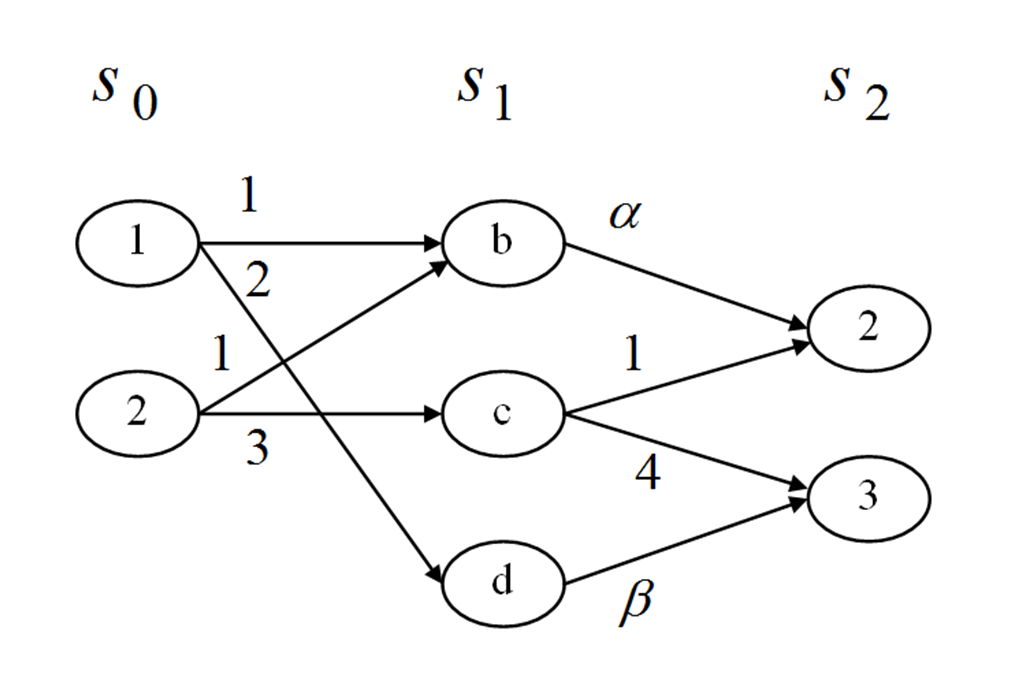
\includegraphics[width=0.5\textwidth]{lecture2_decision_graph}\\
\end{centering}

Here:
\begin{itemize}
  \item $N = 2$, ${S_0} = \{ 1,2\} ,\;{S_1} = \{ b,c,d\} ,\;{S_2} = \{ 2,3\} $,
  \item ${A_0}(1) = \{ 1,2\} $, ${A_0}(2) = \{ 1,3\} $, ${A_1}(b) = \{ \alpha \} $, ${A_1}(c) = \{ 1,4\} $, ${A_1}(d) = \{ \beta \} $
  \item ${f_0}(1,1) = b,\;{f_0}(1,2) = d,\;{f_0}(2,1) = b,\;{f_0}(2,3) = c$, ${f_1}(b,\alpha ) = 2$, etc.
\end{itemize}

\begin{definition}{\textbf{Feasible Path}} \\
A feasible path for the specified system is a sequence $({s_0},{a_0}, \ldots ,{s_{N - 1}},{a_{N - 1}},{s_N})$ of states and actions, such that ${a_k} \in {A_k}({s_k})$ and ${s_{k + 1}} = {f_k}({s_k},{a_k})$.

\vspace{10pt}
\begin{centering}
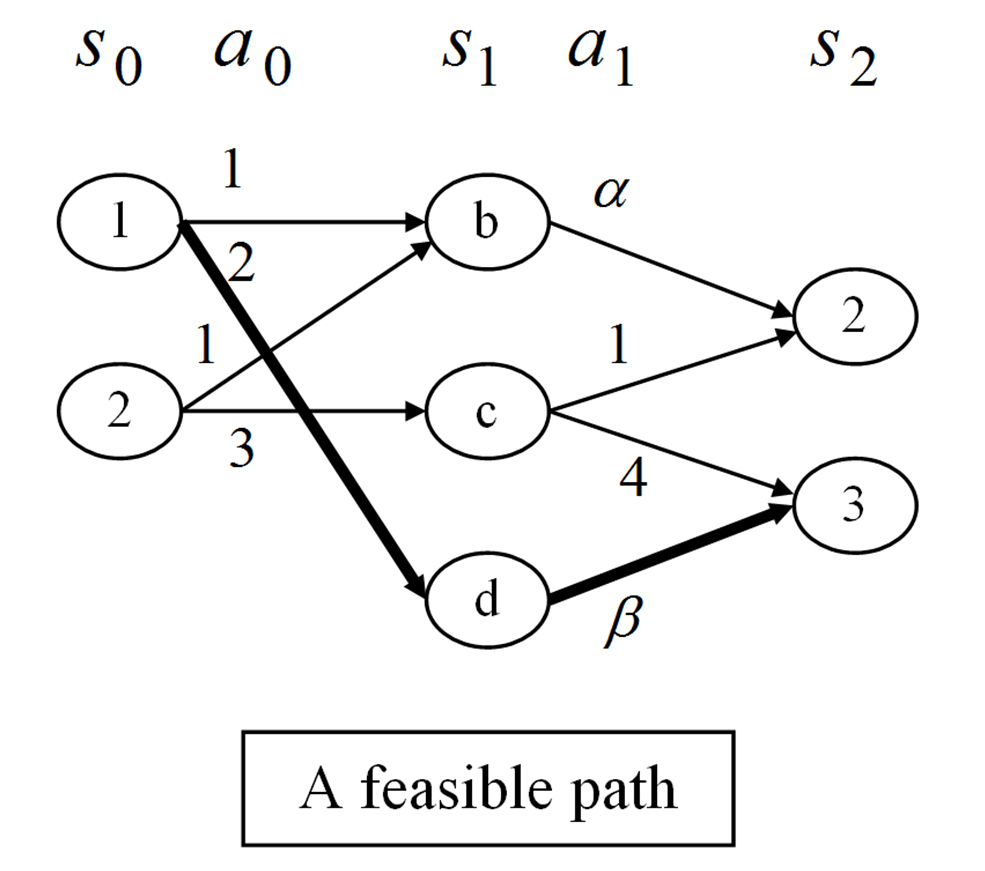
\includegraphics[width=0.4\textwidth]{lecture2_feasible_path}\\
\end{centering}
\end{definition}

\section{The Finite Horizon Decision Problem}

We proceed to define our first and simplest planning problem. For that we need to specify a \emph{performance objective} for our model, and the notion of \emph{control policies}.

\subsection{Costs and Rewards}

\paragraph{The cumulative cost:}  Let ${h_N} = ({s_0},{a_0}, \ldots ,{s_{N - 1}},{a_{N - 1}},{s_N})$ denote an $N$-stage path for the system. To each feasible path ${h_N}$ we wish to assign some cost ${C_N} = {C_N}({h_N})$.

The standard definition of the cost ${C_N}$ is through the following \emph{cumulative cost functional}:
\[{C_N}({h_N}) = \sum\limits_{k = 0}^{N - 1} {{c_k}({s_k},{a_k}) + {c_N}({s_N})} \]

Here:
 	\begin{itemize}
    \item ${c_k}({s_k},{a_k})$ is the \emph{instantaneous}  cost or \emph{single-stage }cost at stage $k$, and ${c_k}$ is the instantaneous cost function.
    \item ${c_N}({s_N})$ is the \emph{terminal} cost, and ${c_N}$ is the terminal cost function.
  \end{itemize}

\paragraph{Note:}
\begin{itemize}
  \item The cost functional defined above is \emph{additive} in time. Other cost functionals are possible, for example the max cost, but additive cost is by far the most common and useful.
  \item We shall refer to ${C_N}$ as the \emph{cumulative $N$-stage cost}, or just the \emph{cumulative cost}.
\end{itemize}

Our objective is to \emph{minimize} the cumulative cost ${C_N}$, by a proper choice of actions. We will define that goal more formally below.

\paragraph{Cost versus reward formulation: }It is often more natural to consider \emph{maximizing} reward rather than minimizing cost.  In that case, we define the cumulative $N$-stage return function:
$${R_N}({h_N}) = \sum\limits_{k = 0}^{N - 1} {{r_k}({s_k},{a_k}) + {r_N}({s_N})} $$
Here ${r_k}$ is the running reward, and ${r_N}$ is the terminal reward.
Clearly, minimizing ${C_N}$ is equivalent to maximizing ${R_N}$, if we set:
$${r_k}(s,a) =  - {c_k}(s,a) \text{ and }{r_N}(s) =  - {c_N}(s).$$


\subsection{Optimal Paths}

Our first planning problem is the following \emph{Path Optimization Problem}:
\begin{itemize}
  \item For a given initial state ${s_0}$, find a feasible path ${h_N} = ({s_0},{a_0}, \ldots ,{s_{N - 1}},{a_{N - 1}},{s_N})$ that minimizes the cost functional ${C_N}({h_N})$, over all feasible paths ${h_N}$.
\end{itemize}

Such a path is called an \emph{optimal path} from ${s_0}$.

A more general notion than a path is that of a \emph{control policy}, that specifies the action to be taken at each state. Control policies will play an important role in our Dynamic Programming algorithms, and are defined next.

\subsection{Control Policies}

\begin{definition} A control policy, denoted $\pi $, specifies for each state a unique action to be taken at this state. Specifically, a control policy  $\pi $ is a sequence $\pi  = ({\pi _0}, \ldots ,{\pi _{N - 1}})$ of decision functions, where
${\pi _k}:{S_k} \to {A_k}$,    and  ${\pi _k}(s) \in {A_k}(s)$.
The action to be taken at time $k$ in state ${s_k}$ is given as
${a_k} = {\pi _k}({s_k})$
\end{definition}

\paragraph{Classes of control policies}
Observe that we allow the function ${\pi _k}$ policy to depend on the time $k$. Such time-dependent policies are also called \emph{non-stationary}. On the other hand, we confine ourselves here to policies that are:
\begin{itemize}
  \item \textbf{Markovian}: The action ${a_k}$ is a function of the current state ${s_k}$ only, and not on previous states and actions. Non-Markovian policies: also called history-dependent policies, will be extensively used in the learning part of the course.
  \item \textbf{Deterministic}: More general policies may use randomization in the selection of actions. Such randomized policies are also used in learning algorithms, as well as in game problems.
\end{itemize}

\paragraph{Control policies and paths:} As mentioned, a control policy specifies an action for each state, whereas a path specifies an action only for states along the path. This distinction is illustrated in the following figure.

\begin{centering}
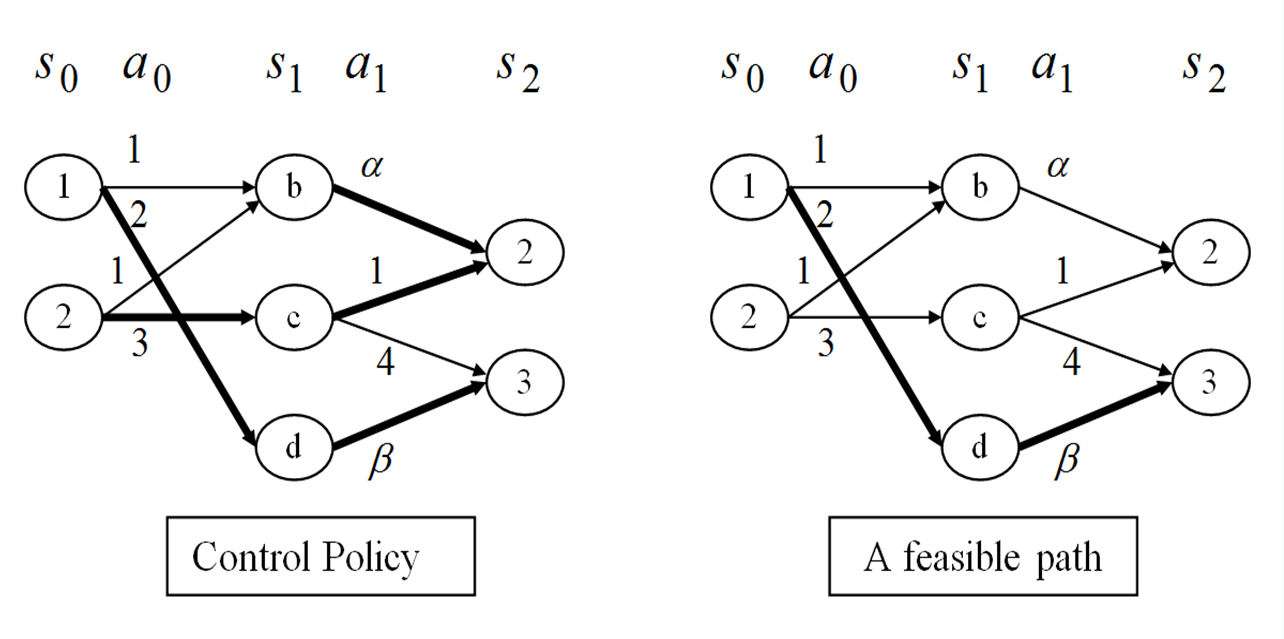
\includegraphics[width=0.8\textwidth]{lecture2_policy_path}\\
\end{centering}

\paragraph{Induced Path:} A control policy $\pi $, together with an initial state ${s_0}$, specify a feasible path ${h_N} = ({s_0},{a_0}, \ldots ,{s_{N - 1}},{a_{N - 1}},{s_N})$. This path may be computed recursively using ${a_k} = {\pi _k}({s_k})$ and ${s_{k + 1}} = {f_k}({s_k},{a_k})$, for $k = 0,1, \ldots ,N - 1$.

\begin{remark} Suppose that for each state ${s_k}$, each action ${a_k} \in {A_k}({s_k})$ leads to a different state ${s_{k + 1}}$ (i.e., at most one edge connects any two states). We can then identify each action ${a_k} \in {A_k}(s)$ with the next state ${s_{k + 1}} = {f_k}(s,{a_k})$ it induces. In that case a path may be uniquely specified by the state sequence $({s_0},{s_1}, \ldots ,{s_N})$.
\end{remark}

\subsection{Optimal Control Policies}

\begin{definition} A control policy $\pi $ is called \textbf{optimal} if, for each initial state ${s_0}$, it induces an optimal path ${h_N}$ from ${s_0}$.
\end{definition}

An alternative definition can be given in terms of policies only. For that purpose, let ${h_N}(\pi ;{s_0})$ denote the path induced by the policy $\pi $ from ${s_0}$.  For a given return  functional ${R_N}({h_N})$, denote
${R_N}(\pi ;{s_0}) = {R_N}({h_N}(\pi ;{s_0}))$
That is, ${R_N}(\pi ;{s_0})$ is the cumulative return for the path induced by by $\pi $ from ${s_0}$.

\begin{definition} A control policy $\pi $ is called optimal if, for each initial state ${s_0}$, it holds that ${R_N}(\pi ;{s_0}) \ge {R_N}(\tilde \pi ;{s_0})$
for any other policy $\tilde \pi $.
\end{definition}

Equivalence of the two definitions can be easily established (exercise). An optimal policy is often denoted by ${\pi ^*}$.

\vspace{10pt}
\fbox{\begin{minipage}{0.9\textwidth}
\textbf{The standard finite-horizon planning problem:}  Find an optimal control policy ${\pi ^*}$ for the $N$-stage decision problem with the cumulative return (or cost) function.
\end{minipage}}


\normalsize
\paragraph{The naive approach to finding an optimal policy:}  For finite models (i.e., finite state and action spaces), the number of feasible paths (or control policies) is finite.  It is therefore possible, in principle, to enumerate all N-stage paths, compute the cumulative return for each one, and choose the one which gives the largest return.
Let us evaluate the number of different paths and control policies.
Suppose for simplicity that number of states at each stage is the same: $|{X_k}| = n$, and similarly the number of actions at each state is the same: $|{A_k}(x)| = m$ (with $m \le n$) . The number of feasible N-stage paths for each initial state is seen to be ${m^N}$. The number of different policies is ${m^{nN}}$.
For example, for a fairly small problem with $N = n = m = 10$, we obtain ${10^{10}}$ paths for each initial state (and ${10^{11}}$ overall), and ${10^{100}}$ control policies. Clearly it is not possible to enumerate them all.

Fortunately, Dynamic Programming offers a drastic simplification of the computational complexity for this problem.

\section{Finite Horizon Dynamic Programming}

The Dynamic Programming (DP) algorithm breaks down the $N$-stage decision problem into $N$ sequential single-stage optimization problems. This results in dramatic improvement in computation efficiency.

The DP technique for dynamic systems is based on a general observation called Bellman's Principle of Optimality. Essentially it states the following (for deterministic problems):
\begin{itemize}
  \item \textbf{Any sub-path of an optimal path is itself an optimal path between its end points.}
\end{itemize}

Applying this principle recursively from the last stage backward, obtains the (backward) Dynamic Programming algorithm. Let us first illustrate the idea with following example.

\begin{example} Shortest path on a decision graph:  Suppose we wish to find the shortest path (minimum cost path) from the initial node in $N$ steps.

\begin{centering}
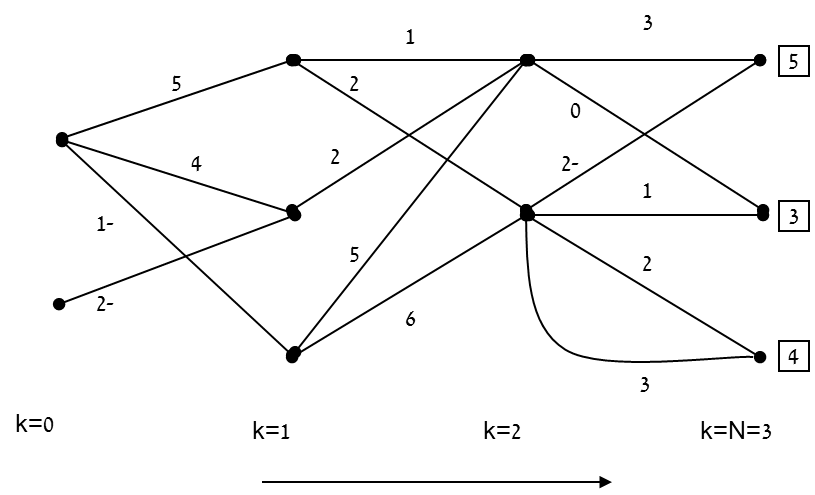
\includegraphics[width=0.8\textwidth]{lecture2_DP}
\end{centering}
\\
The boxed values are the terminal costs at stage $N$, the other number are the link costs.
Using backward recursion, we may obtain that the minimal path costs from the two initial states are 7 and 3, as well as the optimal paths and an optimal policy.

\end{example}

We can now describe the DP algorithm. Recall that we consider the dynamic system
$${s_{k + 1}} = {f_k}({s_k},{a_k}),\quad k = 0,1,2, \ldots ,N - 1$$
$${s_k} \in {S_k},\quad {a_k} \in {A_k}({s_k})$$
and we wish to maximize the cumulative return:
$${R_N} = \sum\limits_{k = 0}^{N - 1} {{r_k}({s_k},{a_k}) + {r_N}({s_N})} $$
The DP algorithm computes recursively a set of \textbf{value functions} $V_k^{}:{S_k} \to \R$ , where $V_k^{}({s_k})$ is the value of an optimal sub-path ${h_{k:N}} = ({s_k},{a_k}, \ldots ,{s_N})$ that starts at ${s_k}$.

\begin{algorithm_}
\textbf{Finite-horizon Dynamic Programming}
\begin{enumerate}
  \item Initialize the value function:   $V_N^{}(s) = {r_N}(s)$,  $s \in {S_N}$.
  \item Backward recursion:  For $k = N - 1, \ldots ,0$, compute
\[V_k^{}(s) = \mathop {\max }\limits_{a \in {A_k}} \left\{ {{r_k}(s,a) + V_{k + 1}^{}({f_k}(s,a))} \right\},\quad     s \in {S_k}.\]
  \item Optimal policy: Choose any control policy $\pi  = ({\pi _k})$ that satisfies:
\[\pi _k^{}(s) \in \mathop {\arg \max }\limits_{a \in {A_k}} \left\{ {{r_k}(s,a) + V_{k + 1}^{}({f_k}(s,a))} \right\},\quad      k = 0, \ldots ,N - 1.\]
\end{enumerate}
\end{algorithm_}

\begin{proposition}
The following holds for finite-horizon dynamic programming:
\begin{enumerate}
  \item The control policy $\pi $ computed above is an optimal control policy for the $N$-stage decision problem.
  \item $V_0^{}(s)$ is the optimal N-stage return from initial state ${s_0} = s$:
\[{V_0}(s) = \mathop {\max }\limits_\pi  {R_N}(\pi ;s),\;\quad \forall s \in {S_0}.\]
\end{enumerate}
\end{proposition}

We will provide a proof of this result in a later lecture, for the more general stochastic MDP model. For the time being, let us make the following observations:
\begin{enumerate}
  \item The algorithm involves visiting each state exactly once, proceeding backward in time. For each time instant (or stage) $k$, the value function ${V_k}(s)$ is computed for all states $s \in {S_k}$ before proceeding to stage $k - 1$.
  \item The recursive equation in part 2 of the algorithm, along with similar equations in the theory of DP, is called \textbf{Bellman's equation}.
  \item Computational complexity: There is a total of $nN$ states (excluding the final one), and in each we need $m$ computations. Hence, the number of required calculations is $mnN$.
For the example above with $m = n = N = 10$, we need $O({10^3})$ calculations.
  \item A similar algorithm that proceeds forward in time (from $k = 0$ to $k = N$) can be devised. We note that this will not be possible for stochastic systems (i.e., the stochastic MDP model).
  \item The celebrated \textbf{Viterbi algorithm} is an important instance of finite-horizon DP. The algorithm essentially finds the most likely sequence of states in a Markov chain $({s_k})$ that is partially (or noisily) observed.
The algorithm was introduced in 1967 for decoding convolution codes over noisy digital communication links. It has found extensive applications in communications, and is a basic computational tool in Hidden Markov Models (HMMs), a popular statistical model that is used extensively in speech recognition and bioinformatics, among other areas.
\end{enumerate}

\paragraph{Historical Notes:}
\begin{itemize}
  \item Dynamic Programming was popularized in the 1950's and 1960's by \textbf{Richard Bellman} (1920-1984), an American mathematician (of Jewish descent). Bellman, who coined the term Dynamic Programming, formulated the general theory and proposed numerous applications in control and operations research.
  \item \textbf{Andrew Viterbi} (born 1935) is an American professor of electric engineer, a pioneer in the field of digital communications, and co-founder of Qualcomm Inc. (together with Irwin Jacobs). He has had close ties with the Technion, and has made many contributions to our department.
\end{itemize}




%\end{document}

